\chapter{Results and Discussion}

\section{Introduction}
This Chapter describes and evaluates the data collected during the execution states (both local and HPC). The evaluation of the RAG-variants implemented locally will be performed with respect to timing, as well as on the quality of the retrieved and given answers, which have been specified in chapters 4 and 5. 

% TODO: write about HPC as well

\section{Results of the Local Runs }
For the six local versions: (1) an in memory version, (2) a Milvus based version, (3) a Milvus based version which has been optimized (tuned), (4) a dense reranking version, (5) a hybrid-retrieval version, and finally (6) a version where both reranking and hybrid-retrieval are combined, we have the following results:

\begin{table}[htbp]
    \centering
    \caption{Summary of local evaluation results averaged across the five scenarios.}
    \label{tab:local-results-summary}
    \resizebox{\textwidth}{!}{%
    \begin{tabular}{lrrrrrr}
        \toprule
        Implementation & Manual & Ret. F1 & Index & Retrieve & Generate & Answer len. \\
        \midrule
        Basic & 0.80 & 0.424 & 17.65 & 0.067 & 27.47 & 147.0 \\
        VectorDB & 0.60 & 0.451 & 35.43 & 0.104 & 21.95 & 104.0 \\
        VectorDB tuned & 0.60 & 0.366 & 36.87 & 0.103 & 31.67 & 120.8 \\
        Reranker & 0.50 & 0.345 & 57.69 & 1.148 & 28.31 & 85.8 \\
        Hybrid & 0.40 & 0.279 & 34.87 & 0.175 & 25.52 & 116.4 \\
        Hybrid rerank & 0.60 & 0.405 & 62.96 & 2.988 & 35.79 & 119.0 \\
        \bottomrule
    \end{tabular}
    }
\end{table}

As indicated by Table~\ref{tab:local-results-summary}, the best results for both manual answer scores (answer quality) and retrieval F1 (retrieval quality), were obtained using different pipelines. Thus it is clear that while there was a correlation between these two aspects of overall pipeline performance, they are not synonymous. It may be possible to obtain high-quality retrieved content in terms of relevance, but fail to generate the complete or correct answer due to the lack of detail selection during generation.

\subsection{Local Timing Comparison}
Figure~\ref{fig:timing-breakdown} illustrates the average execution time for each of the local runs. The simplest in-memory pipeline was able to index faster than all other configurations with an average of 17.65 seconds. The pipelines that utilized a Milvus backend took longer to index since the document chunks and their corresponding embeddings were being stored on an outside vector data base. The reranking and hybrid-reranking pipelines had the longest indexing times (57.69 and 62.96 seconds) as these are configured to perform additional retrieval operations and therefore have a greater number of steps within their setups.

\begin{figure}[htbp]
    \centering
    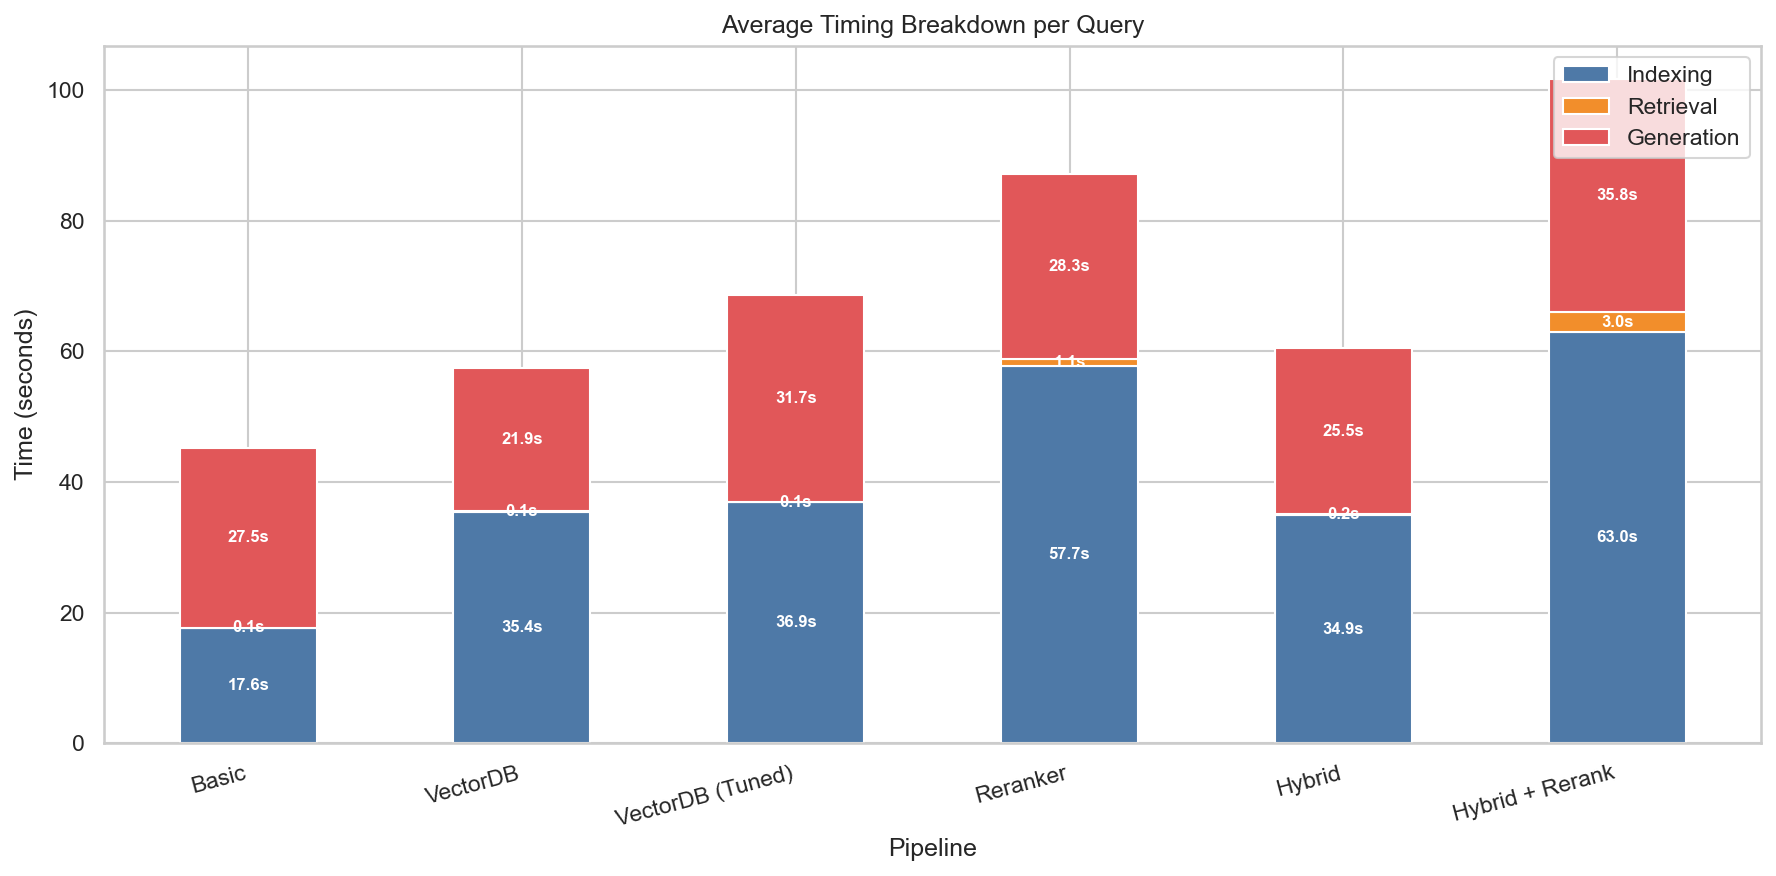
\includegraphics[width=\textwidth]{images/fig11_timing_breakdown.png}
    \caption{Average local timing breakdown for indexing, retrieval, and generation across the implemented RAG variants.}
    \label{fig:timing-breakdown}
\end{figure}

Retrieval times were very short for all three of our query-pipelines (the "basic" pipeline, the "original" vector database pipeline, and the "tuned" vector database pipeline). The Basic pipeline took on average 0.067 seconds, the Original Vector Database Pipeline took on average about 0.104 seconds, and the Tuned Vector Database Pipeline took on average about 0.103 seconds. The use of a Hybrid Retrieval method resulted in longer retrieval times with an average of 0.175 seconds and, as expected, Reranking caused longer retrieval times since another cross encoder pass was made to the Candidate Set. The longest retrieval time was from the Hybrid-Reranking Pipeline with an average of 2.988 seconds.

The Generation Times for each of the implementations were greater than the Retrieval Times for each of the implementations. The Tuned Vector-Database Pipeline had the least amount of Average Generation Time with an average of 21.95 seconds and the Hybrid-Reranking Pipeline had the largest Average Generation Time with an average of 35.79 seconds. This indicates that in this local environment, the Language Model Generation Step dominated the Per-Query Response Cost. Thus, although retrieval optimization is important, the latency difference was substantially less than that due to Generation Latency, other than when using a Hybrid-Reranking Pipeline.

\subsection{Local Retrieval and Answer Quality}
Figure ~\ref{fig:answer-quality} provides an answer-quality comparison. Of the pipelines shown in Figure \ref{fig:answer-quality}, the Basic Pipeline received the highest Manual Score at 0.80 which included 2 \textit{Correct Answers} and 1 \textit{Partially-Correct Answer}. All other pipelines had scores that were lower than the Basic Pipeline. Vector-Database had a score of 0.60 as did Tuned Vector Database and Hybrid-Reranking. Reranking had a score of 0.50 while Hybrid was slightly lower with a score of 0.40.

\begin{figure}[htbp]
    \centering
    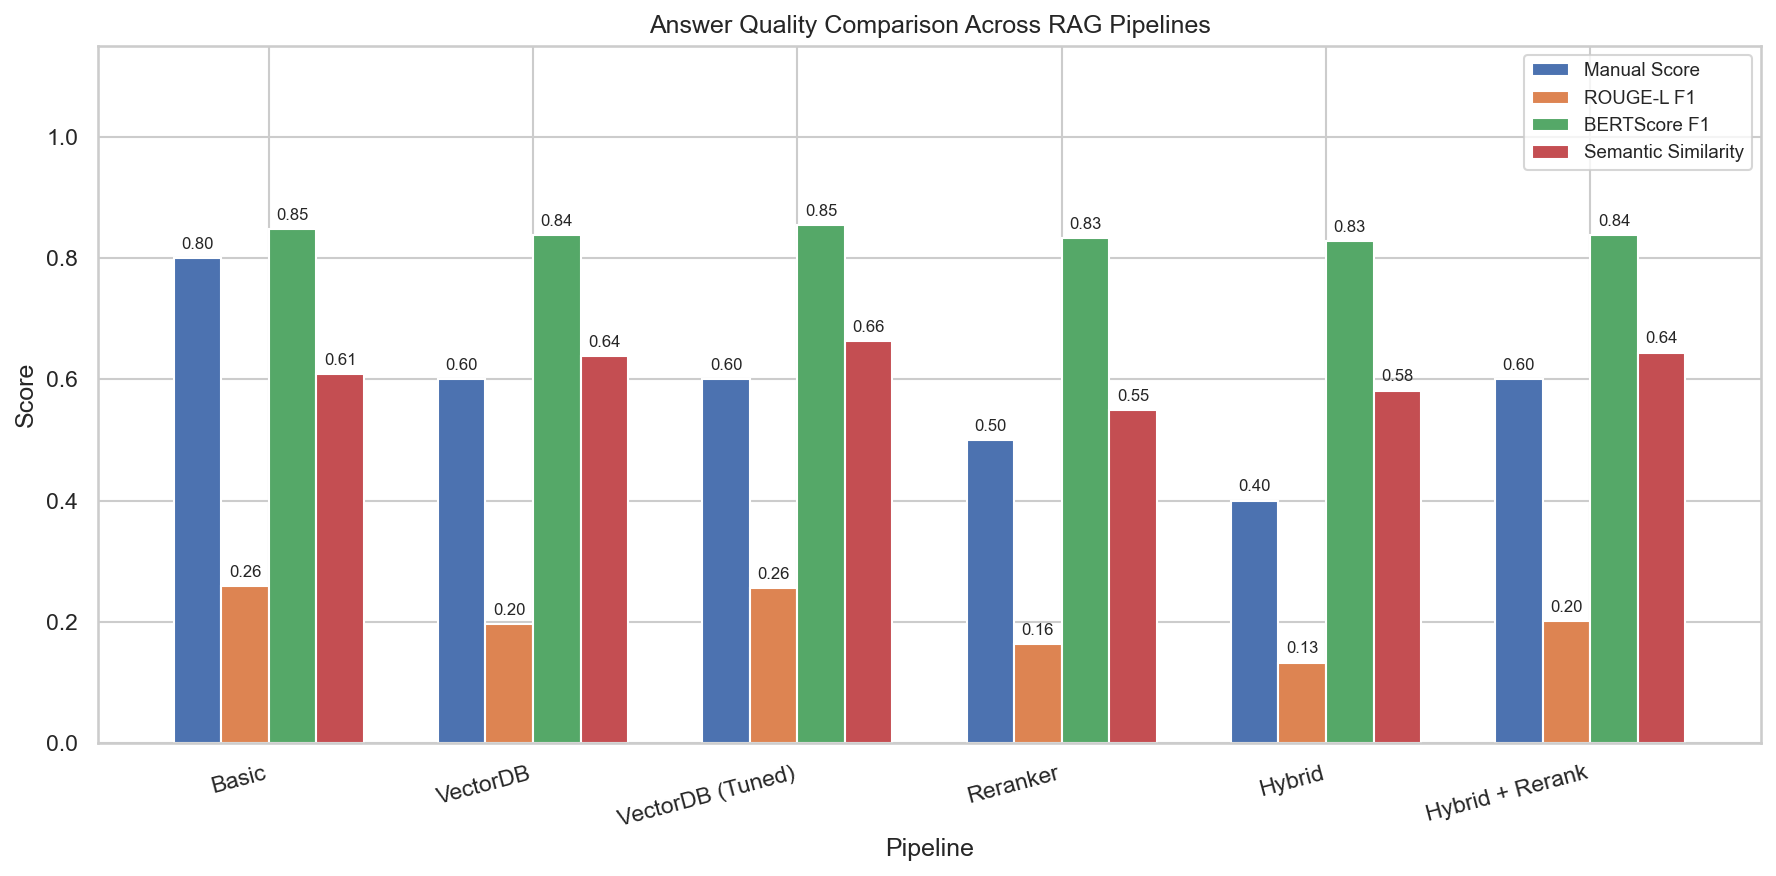
\includegraphics[width=\textwidth]{images/fig09_answer_quality.png}
    \caption{Answer-quality metrics for the local RAG variants, including manual score, ROUGE-L, BERTScore, and semantic similarity.}
    \label{fig:answer-quality}
\end{figure}

The results from using automatic semantic metrics did not always match up perfectly to the manual scores. For example, although the manually-tuned version of the vector-database pipeline got the highest BERTScore and semantic-similarity (which both reward how much information overlaps with a given reference-answer) it only received a manual-score of 0.60. There are two reasons for this discrepancy. First, semantic-similarity only looks at how much information in your response overlaps with the information in the reference answer. Second, when doing manual-scoring we look to see if you provided enough detail about each operation, or if you left anything out.

As shown in Figure ~\ref{fig:retrieval-quality}, the vector-database-pipeline produced the best results for all retrieval-based metrics. It scored an F1 of 0.451, which represented the highest value for that metric; and it also scored a precision of 0.319, again representing the highest value for that metric. The basic-pipeline scored an F1 of 0.424, and hybrid-reranking scored an F1 of 0.405. All four of those pipelines (basic-pipeline, vector-database-pipeline, tuned-vector-database-pipeline, and hybrid-reranking) scored a perfect 100\% on retrieval-recall. The reranker scored 90\%, and the hybrid-pipeline scored 70\%.

\begin{figure}[htbp]
    \centering
    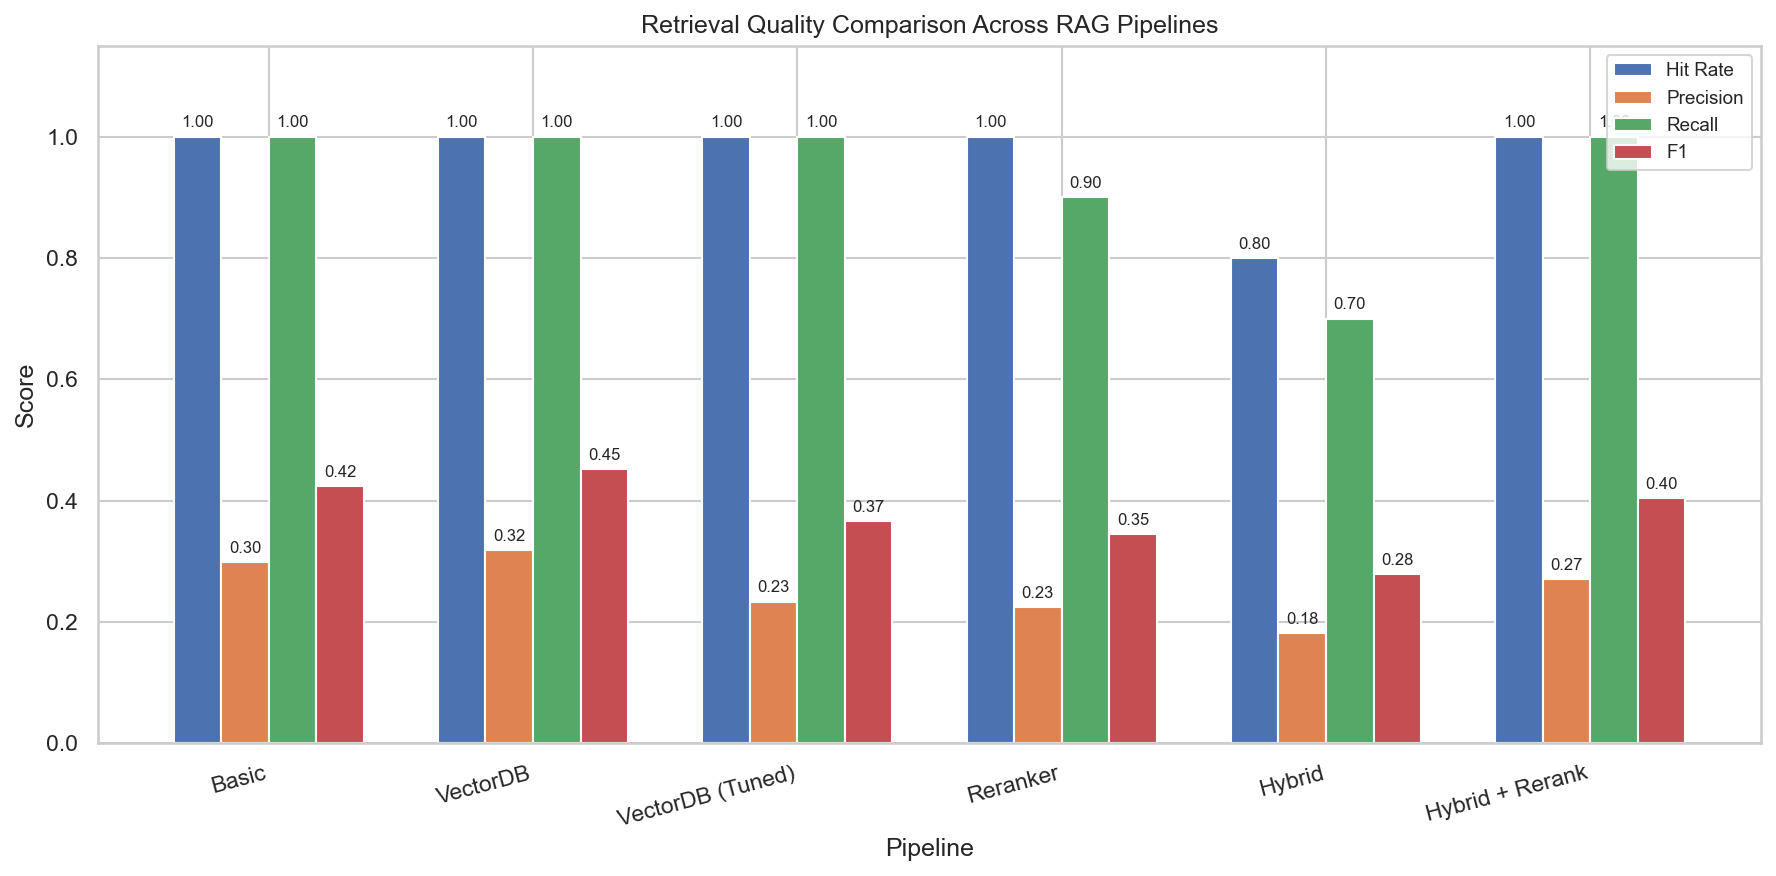
\includegraphics[width=\textwidth]{images/fig10_retrieval_quality.png}
    \caption{Retrieval-quality metrics for the local RAG variants, comparing hit rate, precision, recall, and F1.}
    \label{fig:retrieval-quality}
\end{figure}

The results from this local test indicate that hybrid pipeline performance did not improve overall search quality. Hybrid search is expected to improve performance as a combination of both lexical and semantic cues can enhance search results. However, neither the Milvus hybrid configuration nor the small number of scenarios used in this study provided a significant improvement over the dense-vector database-pipeline.

Hybrid-reranking variant had improved the retrieval-quality in comparison to the hybrid-only, however, there was also a large increase in the time for retrieving results.

Manual score-by-scenario for Figure~\ref {fig:scenario-heatmap} shows that scenario 1, Sev-1 SLA Lookup, was the least difficult (average score = .92). Scenario 3 and 5 were the most difficult (both averaged .42) as they required cross-functionally reasoning of onboarding, IT, Logistics, Customer Success, Product and Commercial. Low scores suggest that searching for the correct documents is insufficient if the user needs information regarding multiple operationally dependent processes.

\begin{figure}[htbp]
    \centering
    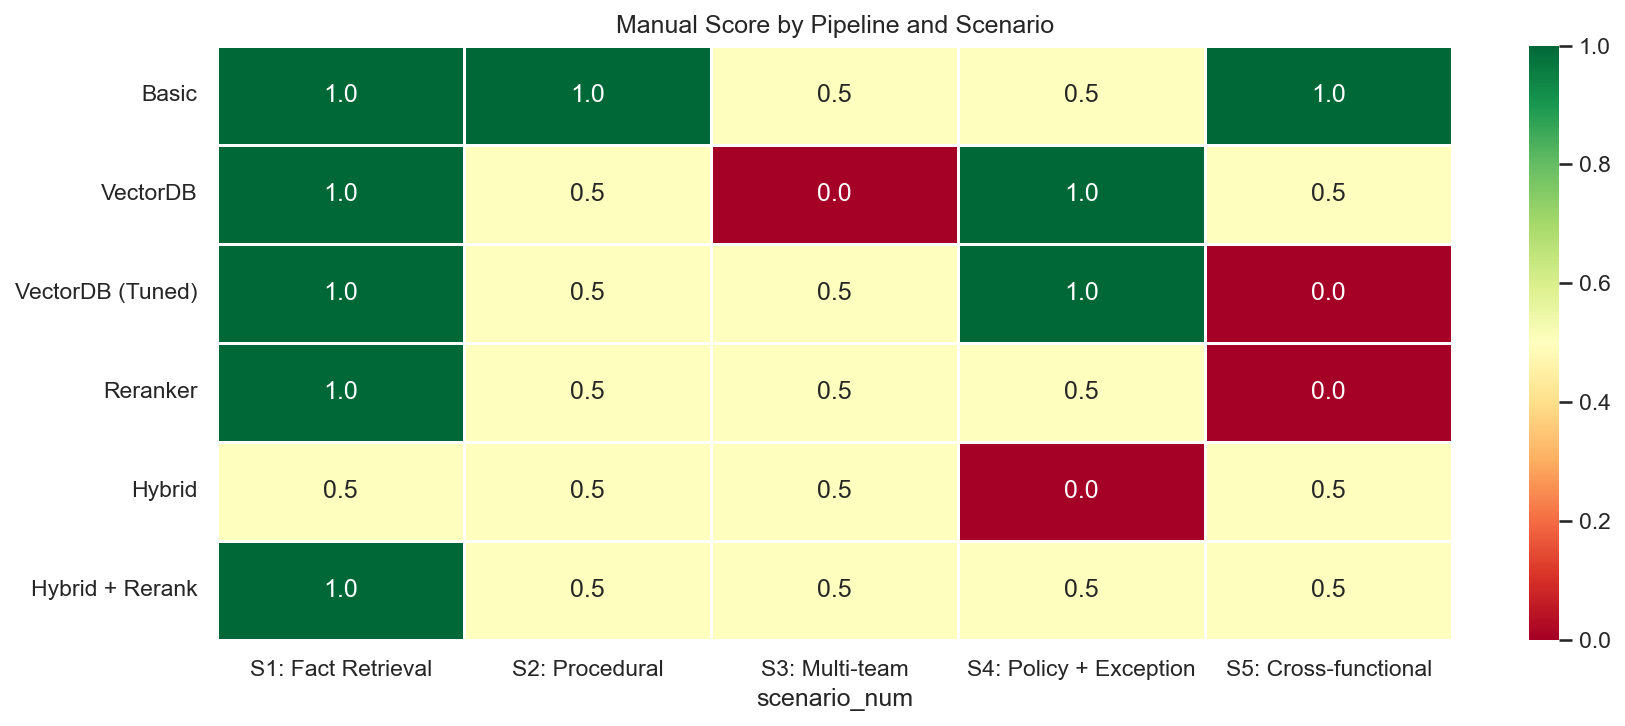
\includegraphics[width=0.92\textwidth]{images/fig12_scenario_heatmap.png}
    \caption{Manual answer score by implementation and scenario. Darker cells indicate stronger manually evaluated answers.}
    \label{fig:scenario-heatmap}
\end{figure}

\begin{figure}[htbp]
    \centering
    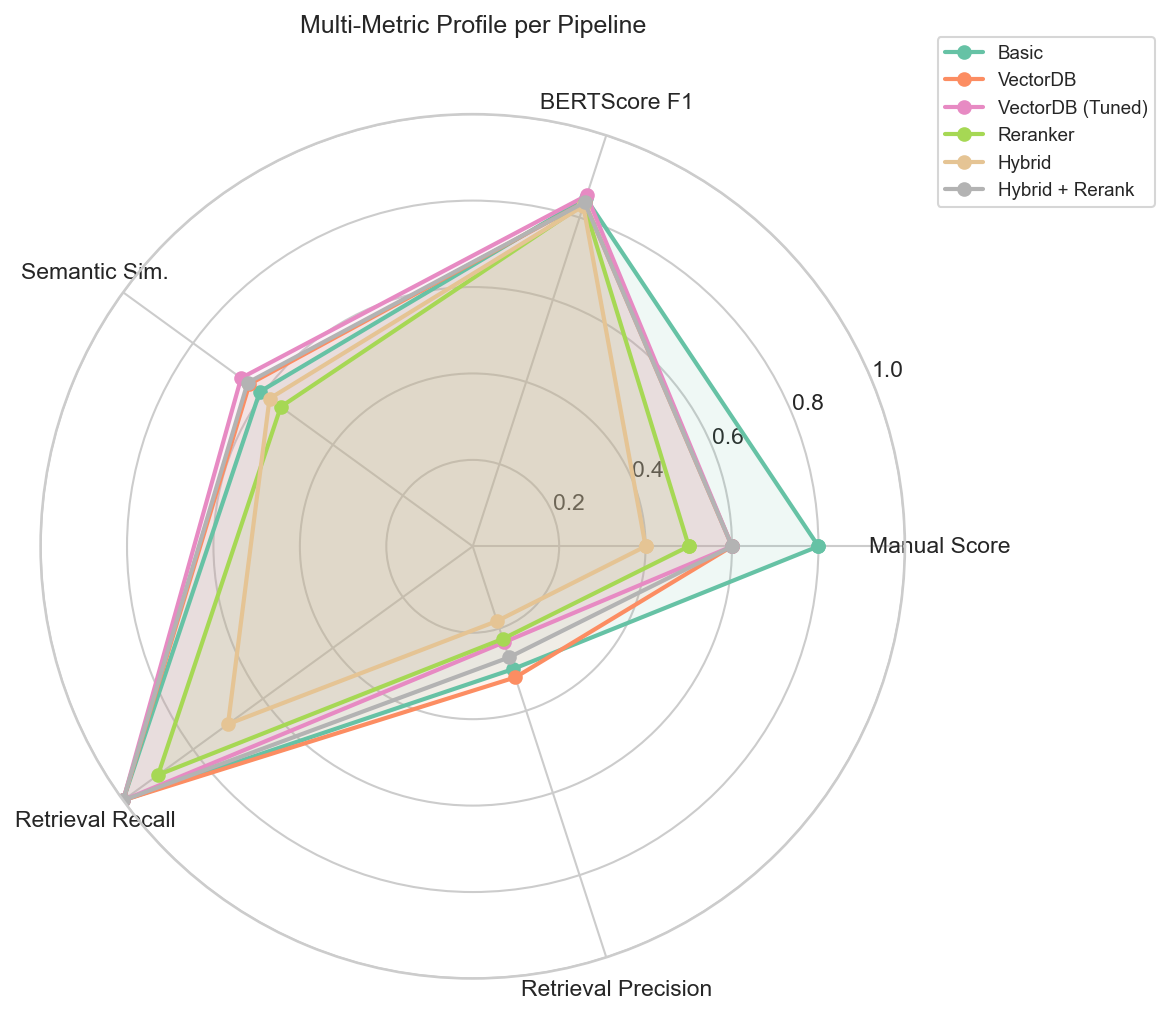
\includegraphics[width=0.85\textwidth]{images/fig13_radar_chart.png}
    \caption{Multi-metric profile of the local RAG pipelines, comparing manual score, BERTScore, semantic similarity, retrieval recall, and retrieval precision.}
    \label{fig:radar-chart}
\end{figure}

\section{HPC Deployment Results}

% TODO: Complete this section after the HPC experiments are executed.
% TODO: Add HPC timing results, quality metrics, node details, scheduler settings,
% container setup, storage paths, and service startup overheads.

\section{Local versus HPC Comparison}

% TODO: Complete this section after both local and HPC results are available.
% TODO: Compare each pipeline locally and on HPC using the same scenario IDs,
% implementation names, timing fields, retrieval metrics, and answer-quality metrics.

\section{Effectiveness of Retrieval-Level Optimization Techniques}
Local results showed mixed effectiveness for Retrieval-Level Optimization Techniques. Dense retrieval using milvus-backed vectors enhanced local F1 scores comparing to in-memory baseline but did not improve manual answer score. This suggests that storing vectors persistently provides a stronger foundation for retrieving data without always enhancing generative quality.

The tuned vector-database run yielded better ROUGE-l, BERTScore and semantic similarity than the original vector database run; however it also decreased local retrieval F1 score. Larger chunks may have given the generator more complete context while also making source level retrieval less accurate. This additional support for chunk size being an experimental parameter with meaning, rather than just a technical process choice.

Reranking did not enhance local manual score in this particular experiment and in fact caused average latency of retrieval to go from sub second range to over one second on average. The hybrid-reranking pipeline was better than hybrid retrieval alone and equivalent to the manual score of vector database variant, but had longest times for both retrieval and generation. Thus, there is no doubt as to the cost associated with reranking and its benefit in terms of quality was limited for this corpus and scenario set.

% TODO: Add findings about HPC

\section{Comparison with Literature}
The results confirm the body of literature's observations about how RAG performance varies with both retrieval quality and generation characteristics. For example, the research demonstrates that dense retrieval is very successful for a controlled Enterprise Corpus (especially when the predicted evidence exists in documents describing policies, handbooks etc. with the same semantic content). At the same time, one can observe that having a large number of retrievals does not always result in an entirely accurate answer. Even though some evidence was found, some generated answers failed to include at least one required owner, escalation trigger, or accountability condition (e.g., even if there were many sources which contained information about them). 

The reranked results are consistent with the expected computational cost/latency trade-offs documented in past literature. While cross-encoders may significantly improve candidate ordering, they add significant additional processing beyond what occurred during the first retrieval. Given the constraints of the experimental design (i.e., the size of the source corpus, the length of candidate lists, and the number of different evaluation test cases), expectations include a proportionally greater increase in manual quality evaluations of candidates based upon their use of additional computation.

Hybrid retrieval results were less strong than anticipated. As noted earlier, hybrid retrieval has been presented as a way to combine the benefits of using exact keyword matches along with retrieving relevant documents from a larger source document collection. Nevertheless, achieving the desired performance gains through hybrid retrieval requires careful tuning of parameters including (but certainly not limited to): configuration settings used for hybrid retrieval, source document collection structures, sparsity levels for vectors representing documents, and query types. Therefore, a belief is these local findings provide sufficient justification for cautionary conclusions. Hybrid retrieval should be carefully tuned, evaluated and compared against dense retrieval before being selected for deployment as a replacement for dense retrieval.

% TODO: Add for HPC

\section{Trade-Offs and Limitations}
While there are many theoretical trade-offs between this approach and others (e.g., what trade-offs will occur as the number of documents grows), the most relevant trade-off for the immediate future appears to be that between \textit{infrastructure-realism} and \textit{simplicity}. In other words, while the baseline in-memory pipeline produced both the best manual score and the shortest indexing times, it is certainly less like an actual deployable application. On the other hand, the vector database pipeline took longer to index (i.e. to set up) than the baseline in memory pipeline, but it produced better retrieval results (i.e. stronger F1 values) and a more reasonable storage basis.

There was another trade-off. Namely one between retrieval quality and query-time. As would be expected, reranking (and hybrid reranking) made substantial increases in the time taken to retrieve answers. However, when a comparison was made between hybrid reranking and hybrid retrieval alone, hybrid reranking resulted in slightly better-quality retrievals, even though it did so at a cost of greater query latency. Given these two observations, the trade-off does appear worthwhile to pursue further, however, whether or not to incur this penalty depends on how much value can be placed upon the extra retrieval accuracy.

There are several important limitations of this evaluation. (i) First, since the corpus is artificial (synthetic), and since the scenario-set contains only five questions, the results have little relevance beyond the specific context used here. (ii) Second, because each candidate was evaluated using only a very simple rubric to manually evaluate their output, the scores do not reflect any subtle differences in performance. (iii) Third, since the evaluation of each candidate was performed locally, results depend heavily on the runtime environment of Ollama, the models' initial warmup time, the presence/absence of background processes running during testing, and the current state of the Milvus service. 

% TODO: add HPC tradeoffs, limitations

\section{Summary}

% TODO
